\documentclass[letterpaper]{article}
\usepackage{polyglossia, fontspec}
\usepackage{amsmath, mathtools}
\usepackage{hyperref}
\usepackage{tikz}
\usepackage[margin = 1.5 in]{geometry}

\title{Project on Monoallelic Expression: a Statistical View}
\author{Attila Gulyás-Kovács}
\bibliographystyle{plain}

\begin{document}

\maketitle

\section{Introduction}

The scope of this document is the research project on monoallelic expression
in the human dorsolateral prefrontal cortex (DLPFC); I will refer to it as the
MAE project and the corresponding draft as the MAE manuscript\footnote{working
title: Novel monoallelically-expressed genes and relaxation of imprinting with
advanced age .  See the text of manuscript
\href{https://docs.google.com/document/d/1cWd4UH98SJR5lihDihC0ZO-C_A1-8MQ5COcixxCLzHE/edit?usp=sharing}{under
this link} and the corresponding figures
\href{https://docs.google.com/presentation/d/1YvpA1AJ-zzir1Iw0F25tO9x8gkSAzqaO4fjB7K3zBhE/edit?usp=sharing}{here}}.
The term \emph{allelic exclusion} will refer to mechanisms resulting in mono
or biallelic expression and \emph{imprinting} will denote the parent-of-origin
specific subtype of allelic exclusion.  My goal here is to evaluate the
current state of the this study in order to facilitate discussion and propel
this project to completion.

In the MAE project two kinds of analysis (task) was carried out:
\begin{enumerate}
\item \emph{classification} to call monoallelic expressing genes in each individual
\item \emph{regression}\footnote{Regression at this point means the inference
of the parameters of some regression model while at some later points it will
refer to the model itself.  The meaning will hopefully be clear from the
context.} to assess the impact of explanatory variables that vary across
individuals
\end{enumerate}

In my understanding, the main results and conclusions may be summarized as
follows:
\begin{enumerate}
\item relatively few genes were called strongly significant suggesting the
total number of monoallelically expressed/imprinted genes is consistent with
the earlier conservative estimate of ca.~200~\cite{DeVeale2012} as opposed to
the liberal estimate of ca.~1300~\cite{Gregg2010}
\item the called genes agree well but not completely with previous gene sets
suggesting some variation accross tissue types and/or organisms
\item the called genes varied across individuals; regression using 8 of the called
genes suggests loss of imprinting with age
\end{enumerate}

The present evaluation finds that the first two conclusions are at best
weakened by the lack of estimated error rates of classification.  The third
point stands out as an interesting but only weakly supported novel finding
that calls for improvements in terms of both its statistical significance and
its generality.

Section~\ref{sec:preliminaries} will introduce some quantities and concepts on
the data and their summary statistics used by the MAE project.  In terms of
those statistics, Section~\ref{sec:models} will present some plausible models
of allelic exclusion that are both genome-wide and population-wide.  These are
not considered in the MAE manuscript but I include them here to help formalize
the rather implicitly stated statistical frameworks of the MAE project in
Section~\ref{sec:stat-framework-mae-project}.  That will pave the way for the
reevaluation of the classification results in Section~\ref{sec:error-rates}
and the regression analysis in Section~\ref{sec:extend-regression}.  In both
cases suggestions will be made for reinterpretation of results or reanalysis
of data.

\section{Preliminaries}
\label{sec:preliminaries}

Genome-wide observations on $m$ genes were based on post mortem tissue samples from the DLPFC
(dorsolateral prefrontal cortex) of $n$ individuals. The $n \times p$ design
matrix $X$ contains observations on all individuals and $p$ \emph{explanatory variables} including age of death and psychological condition (e.g.
schizophrenia).

For each (addressable) gene $g$, and for each individual $i$ inferred to be
heterozygous for \(g\), a statistic $S_{ig}$ was used for classification
resulting in the set \(\{S_{ig}\}_{ig}\).  Each $S_{ig}$ was derived from the
SNP-array and RNA-seq data based on read counts that contain any of the
inferred SNPs in the \((i,g)\) pair.  Let \(N_{ig}\) be the total number of
such counts (based on both alleles) and \(H_{ig} = \sum_{s} H'_{is}\), where
\(H'_{is}\) is the greater of the read counts for the two variants at SNP
\(s\); the summation runs over all inferred SNPs \(s\) (for individual \(i\)
and gene \(g\)).  Using the notations just introduced, the definition in the
MAE manuscript reads as
\begin{equation}
\label{eq:S}
S_{ig} = \frac{H_{ig}}{N_{ig}}.
\end{equation}

LOI\_R\footnote{loss of imprinting ratio?} is another statistic defined by the
MAE project, which was utilized in the regression analysis.  I rename it here
to \(T_i\) to emphasize that each \(T_i\) is specific to individual \(i\).
Scrutiny of some R code\footnote{I received Ifat's code from Andy via email on
2/4/16} related to the MAE project revealed that \(T_i\) was defined in terms
of \(\{S_{ig}\}_g\), where \(g\) is one of 8 selected genes among the
previously known imprinted genes that the classification of the MAE project
called as monoallelically expressing.  For each of those genes \(g\) take the
set \(\{S_{ig}\}_i\) across all individuals \(i\) and, based on that, let
\(\hat{F}_g\) be the empirical cumulative distribution function (e.c.d.f.)
evaluated at each data point; note the linear relation of \(\hat{F}_g\) to
ranks of individuals.  Then the definition based on the R code is essentially
\begin{equation}
\label{eq:T}
T \equiv \{T_i\}_i = \frac{1}{2}\left(\sum_{g=1}^8 \hat{F}_g + 1 \right)
\end{equation}

In words, Eq.~\ref{eq:T} shows that the e.c.d.f.~was averaged over the 8
selected genes and after which it was scaled to \([0.5,1]\) presumably in
order to match the same interval as that containing the possible values of
\(S_{ig}\).  Thus \(T\) is gene specific in the sense that it is based on only
8 genes sharing a property (inferred imprinting) but it is also gene
unspecific in that it aggregates \(\{S_{ig}\}_{ig}\) over those genes.  Due to
the limited applicability of \(T\) (only to those 8 genes) I will base on
$\{S_{ig}\}_{ig}$ all statistical models described in
Section~\ref{sec:models}.

There is a second reason motivated by the fact that the classification
analysis of MAE project is entirely based on $\{S_{ig}\}_{ig}$ suggesting to
consider them as
\href{https://en.wikipedia.org/wiki/Sufficient_statistic}{sufficient
statistics} for the model parameter(s) $\theta$.  This means that the complete
data (from the SNP-array and RNA-seq measurements) carry no more information
on $\theta$ than $\{S_{ig}\}_{ig}$ do, so it is sufficient to draw inferences
on \(\theta\) solely from the latter (in combination with $X$, if $X$ is
informative).  It is likely that sufficiency does not hold but will still be
assumed for consistency with the MAE project and the assumption's simplicity.
Sufficiency will not be discussed here further.

\section{Some plausible statistical models}
\label{sec:models}

I will start from the simplest model family, progressing towards generalized
linear models.  Along the way I will list biological-mechanistic assumptions
behind each model family, and sketch various modeling directions to relax some
of those assumptions.

\subsection{The simplest model family}

For all the model families considered here the following assumptions are made
on the mechanism of allelic exclusion
\begin{itemize}
\item $\{S_{ig}\}$ are sufficient statistics for $\theta$
(Section~\ref{sec:preliminaries})
\item individuals are independent of each other with respect to allelic
exclusion
\end{itemize}

In case of the simplest model family, $\{S_{ig}\}_{ig}$ are independently
distributed according to two probability density functions
(p.d.f.)\footnote{Mathematical rigor would require the term probability
\emph{mass} function because each \(S_{ig}\) is discrete but I use p.d.f.~for
technical reasons too esoteric to be exposed here.  \(f\) might also be called
a likelihood function. } $f(\cdot|a)$ and $f(\cdot|b)$, which correspond to
mono and biallelic expression, respectively:
\begin{eqnarray}
\label{eq:two-level}
\{S_{ig}\}_{ig} &\overset{i.i.d.}{\sim}& f(s | \theta_g) \\
\label{eq:two-level-cases}
\theta_g &=&
\begin{dcases*}
a & when $g$ is monoallelically expressed \\
b & when $g$ is biallelically expressed.
\end{dcases*}
\end{eqnarray}

Eq.~\ref{eq:two-level} says that all \(S_{ig}\) are distributed independently
identically (i.i.d.)~according to probability distribution function \(f\)
parametrized by \(\theta_g\) whenever gene \(g\) is monoallelically (or
biallelically) expressed (Eq.~\ref{eq:two-level-cases}).

For this model family the following additional assumptions must be made on
allelic exclusion:
\begin{enumerate}
\item it takes only two levels (resulting in fully biallelic or monoallelic
expression) of the same alleles in all cells on which the data are based on
\item with respect to allelic exclusion all genes $g$ are independent
\item all monoallelically expressed genes are identical, and the
same holds for the biallelic case
\item explanatory variables $X$ (including age) have no impact on allelic
exclusion
\end{enumerate}

\subsection{Directions for generalization}
\label{sec:generalizations}

When the first assumption above is relaxed to allow \emph{multiple levels of allelic exclusion}
within single cells and/or variation among cells, we need a separate
$\theta_G$ parameter for each level to express the strength of allelic
exclusion:
\begin{equation*}
\{S_{ig}\}_{ig} \overset{i.i.d.}{\sim} f(s | \theta_G) \quad \forall g \in G.
\end{equation*}
The difficulty with this model family is twofold.  First, the biological
significance of different levels of $\theta_G$ seems vague.  Second, the
fraction of monoallelically expressed genes (genome-wide or restricted to
addressable genes) cannot be expressed by a single number as in the two level
case  (see \(\pi_1\) in Section~\ref{sec:error-rates}).  Here I will not
pursue this direction further and continue by assuming two levels as before.

\emph{Dependence among genes} (assumption 2.)~is known to exist because of extensive epigenetic
marks for imprinting that span multiple neighboring genes.  The simplest model
family for such dependence is a class of hidden Markov models (HMMs).  Emission probabilities for
\(\theta_{ig}\rightarrow S_{ig}\) are specified by \(f(s | \theta_{ig})\)
(cf.~Eq.~\ref{eq:two-level}), and
the hidden Markov chain is
\(\theta_{i1}\rightarrow\theta_{i2}\rightarrow...\), where each
\(\theta_{ig}\) may only take the two values as in
Eq.~\ref{eq:two-level-cases}.  Neither this direction is followed further
here and I return to the independent genes hypothesis.

\subsection{Regression models}
\label{sec:regression-models}

The following regression models achieve an effect that is similar to
averaging.  Importantly, this model family also allows \(X\) to \emph{impact
allelic exclusion} (assumption 4.).  The simplest model family in this case is
normal linear regression.  Let \(f(\cdot|\mu,\sigma^2)\) denote the
probability density function of the normal distribution with mean
\(\mu\) and variance \(\sigma^2\).  Then for a given individual \(i\)
\begin{eqnarray}
\label{eq:normal-lm}
\{S_{ig}\}_g &\overset{i.i.d.}{\sim}& f(s | x_i \beta_g, \sigma^2_g) \\
\label{eq:shared-regression-param}
\beta_g,\sigma^2_g &=&
\begin{dcases*}
a_1, a_2 & when $g$ is monoallelically expressed \\
b_1, b_2 & when $g$ is biallelically expressed,
\end{dcases*}
\end{eqnarray}
where \(x_i\) is the \(i\)-th row of \(X\) and \(\beta_g\) is a \(p\)-length
vector of regression coefficients.

In this model family the multi level explanatory variables \(x_i\) enter the model specification as
scaling factors of the regression parameters \(\beta_g\).  Therefore \(S_{ig}\) may be distributed
according to many more distributions than just two because \(f\) in Eq.~\ref{eq:normal-lm}
incorporates \(x_i\).  Yet, this model family still allows binary
classification (Section~\ref{sec:extend-regression}) since \(X\) is known
and, as in Eq.~\ref{eq:two-level-cases}, the unknown parameter(s) may only take two values.

Linearity and normality may not hold\footnote{In fact they cannot hold given
the finite sample space of \(S_{ig}\), but assuming them
might be useful.} for \(S_{ig}\) and \(X\).  Generalized linear model
families (among which normal linear models comprise just one family) may offer solutions then.  In
this more general model family Eq.~\ref{eq:normal-lm} modifies to \(\{S_{ig'}\}
\overset{i.i.d.}{\sim} f(s | \theta_{g'}(x_i), \phi_{g'})\), such that \(\theta_{g'}\) is a function
of the explanatory variables \(x_i\), and \(g(\mathrm{E}[S_{ig'}]) = x_i \beta_{g'}\), where \(g\)
is a link function (and \(g'\) denotes some gene).

A further generalization would be to allow direct dependence between the
explanatory variables, e.g.~age of death depends on gender.  This would
require Bayesian networks with the trade-off of higher model complexity.

\section{The statistical frameworks of the MAE project}
\label{sec:stat-framework-mae-project}

The MAE project based its previous classification and regression analysis on
different, though closely related, statistics: \(\{S_{ig}\}_{ig}\)
(Eq.~\ref{eq:S}) and \(T\) (Eq.~\ref{eq:T}), respectively
(Section~\ref{sec:preliminaries}).  Besides that, the two kinds of analysis
differ in their scope, dependencies, model formulation (or the lack of it),
and consequently in parameter estimation and formal hypothesis testing.  These
differences delineate two distinct statistical frameworks, summarized in
Table~\ref{tab:model-used}.  How do these relate to the genome-wide
and population-wide model families introduced in Section~\ref{sec:models}?

\begin{table}[t]
\begin{center}
\begin{tabular}{c|c|c|}
task/analysis & classification & regression on explanatory vars.~\(X\) \\
\hline
goal/question & call monoall.~expr. & impact of \(X\) on allelic exclusion \\
genomic scope & all (addressable) genes & 8 selected monoallelic genes \\
statistic & \(S_{ig}\) & \(T\equiv\{T_i\}_i\) \\
dependencies & \(\{S_{ig}\}_{ig} \overset{i.i.d.}{\sim} f(s |
\theta) \) &
\(T_{i} = x_i \beta + \epsilon_i, \quad \epsilon_i \overset{i.i.d.}{\sim}
\mathcal{N}(0, \sigma^2)\) \\
model family & unspecified \(f\) & normal linear \\
estimation & not done & \(\hat{\beta}, \hat{\sigma}^2\) by least squares \\
formal hypothesis test & not done & evidence for \(\hat{\beta}_\mathrm{age} < 0\) \\
\hline
\end{tabular}
\end{center}
\caption{The statistical framework of the two main tasks of the MAE project }
\label{tab:model-used}
\end{table}

All (addressable) genes in all studied individuals were classified but no
statistical model was formulated for classification.  But if such a model had
been given, it could have belonged to the simple model family in
Eq.~\ref{eq:two-level}-\ref{eq:two-level-cases} for two reasons.  Firstly, two
levels of allelic exclusion were assumed (thus the binary classification).
Secondly, all genes and individuals shared the same set of significance
levels (e.g.~\(S_{ig}>0.9\)), suggesting \(\{S_{ig}\}_{ig}\) may have been
assumed i.i.d., so all monoallelically (or biallelically) expressing genes
within all individuals were considered mechanistically independent and
identical.

If at least the \emph{null distribution} \(f(s|\theta_g=b)\)---the one that
represents the biallelic case in Eq.~\ref{eq:two-level-cases} bottom---had
been specified, binary classification could have been framed as frequentist
hypothesis testing using \(p\)-values and other error rates.  In
Section~\ref{sec:error-rates} I discuss the consequences of classification
without such error rates focusing on two inseparable questions of
classification: (i.)~the number of monoallelically expressed genes and
(ii.)~what fraction of monoallelically called genes are expected to be in fact
biallelic, which is known as false discovery rate (FDR).

In contrast, the regression analysis in the MAE project did specify a model
class.  This is the normal linear family\footnote{implemented in the
\texttt{glm} R function, which was called in Ifat's code without
\texttt{family} argument thus defaulting to \texttt{gaussian}, which is the
normal linear model family.  } explanatory variables \(x_i\) in each
individual \(i\).  But this regression model must be distinguished from
genome-wide and population-wide normal linear models of
Section~\ref{sec:regression-models} on two grounds.  First, in this case only
8 of the imprinted genes were modeled and none of the others (that are either
mono or biallelically expressed, see Eq~\ref{eq:shared-regression-param}).
Second, the response variable in this case was \(T_i\) instead of
\(\{S_{ig}\}_g\), raising two further questions: (i.) is \(T_i\) sufficient
(like \(\{S_{ig}\}_g\) are assumed to be, Section~\ref{sec:preliminaries}),
and (ii.) how is the summation over 8 genes in the definition of \(T_i\)
(Eq.~\ref{eq:T}) affect the inference of parameters \(\beta,\sigma^2\)?
Section~\ref{sec:extend-regression} will elaborate on these questions and
possibly useful extensions to the current regression model.

\section{Classification and its error rates}
\label{sec:error-rates}

\subsection{The inseparability of two questions}

As mentioned above, the classification framework of the MAE project raises
two questions, the first of which is the number of monoallelically expressed genes
or, equivalently, their fraction
\begin{equation}
\label{eq:pi1}
\pi_1 = \frac{\#\{\text{monoallelically expressed genes}\}}{m},
\end{equation}
where \(m\)---as before---is the total number of (addressable) genes.

\begin{figure}[b]
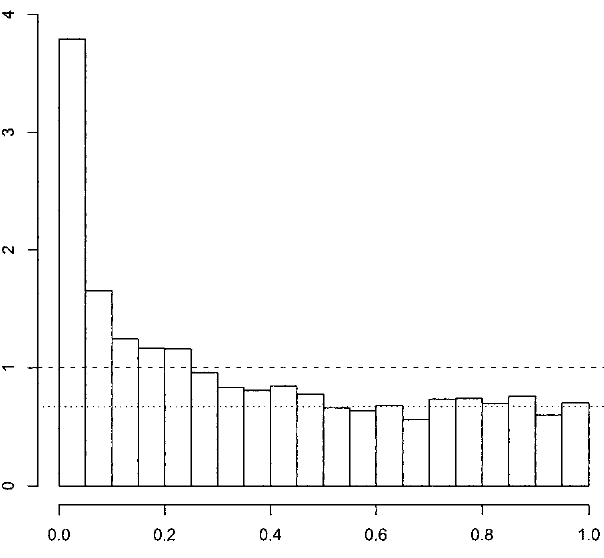
\includegraphics[scale=1.04]{figures/storey-2003-fig1}

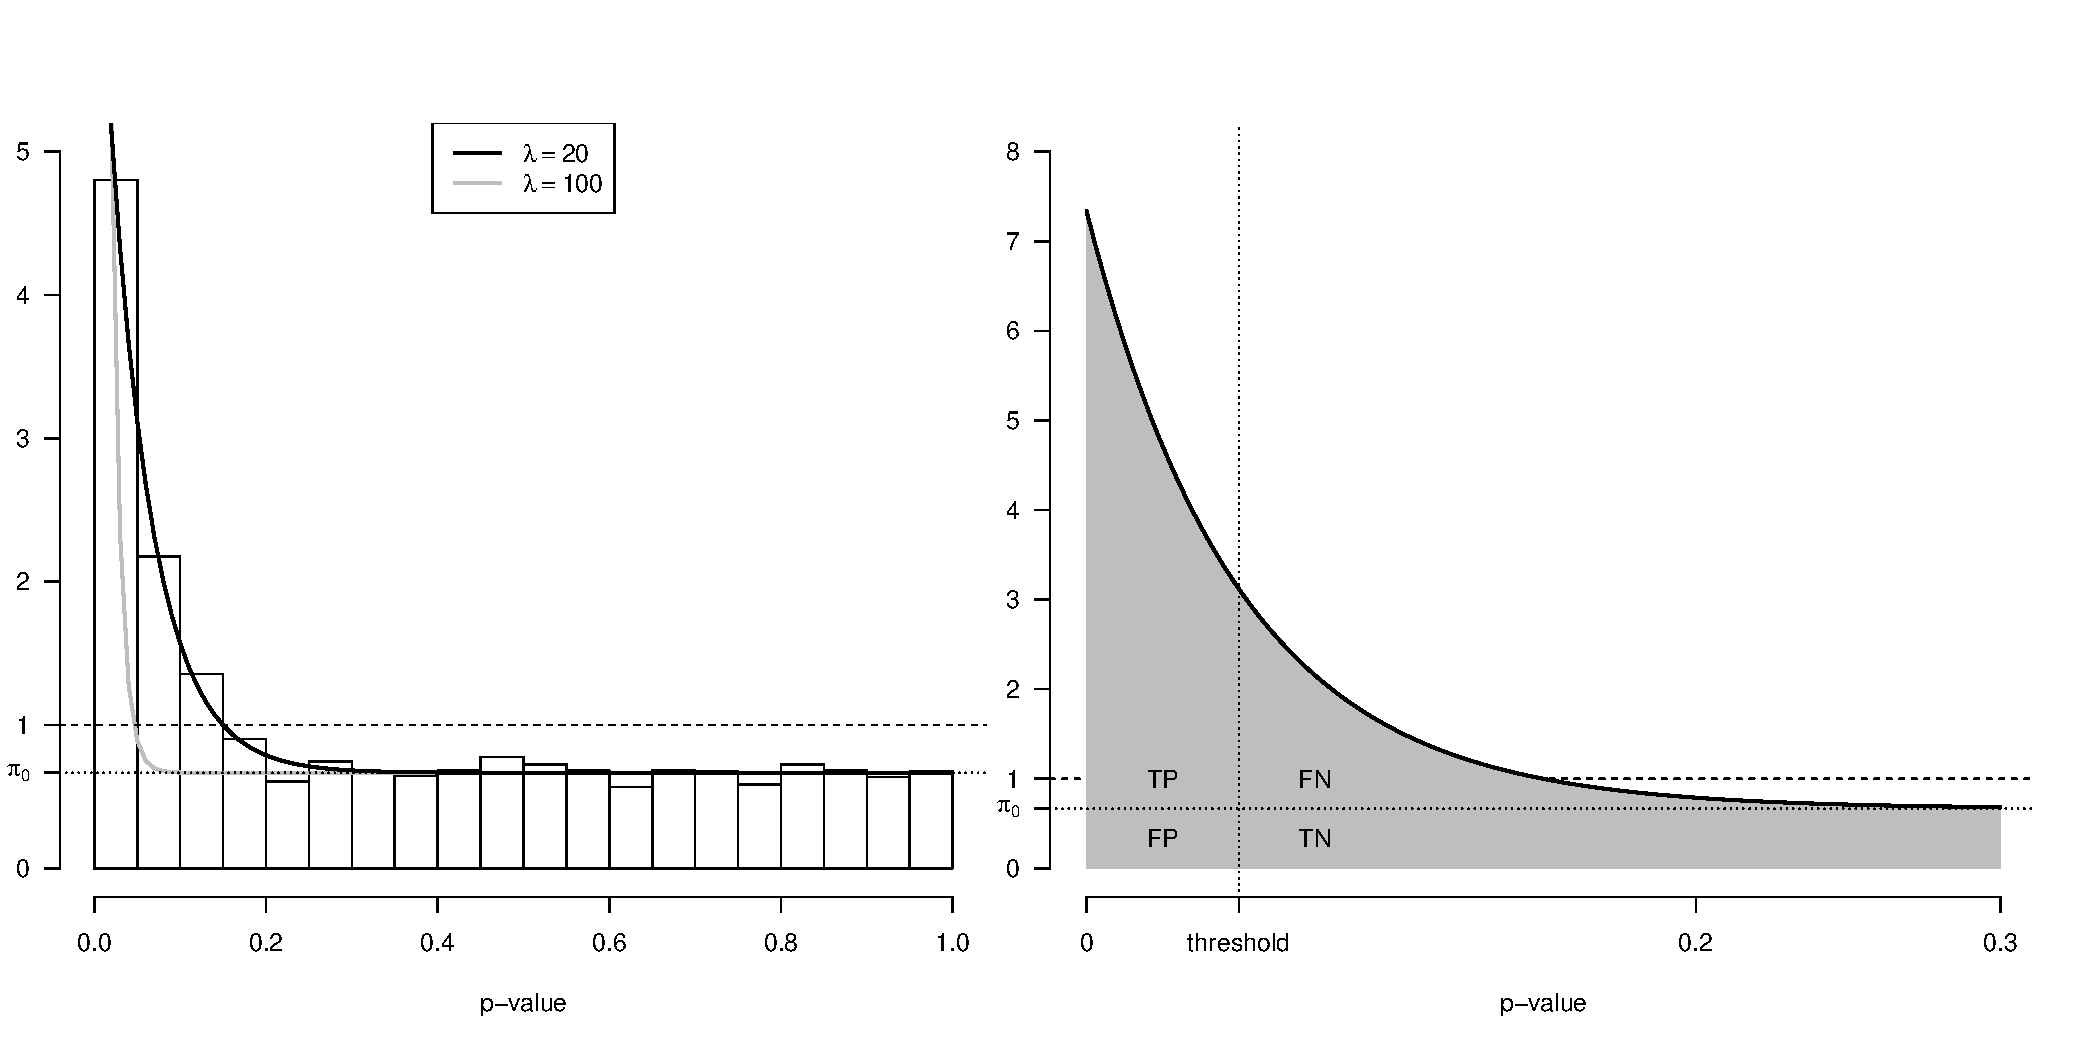
\includegraphics[scale=0.5]{figures/exp-unif-mixture-1.pdf}
\caption{\(\pi_0 : \pi_1\) mixtures of null and alternative distributions of
\(p\)-values.  \emph{Top:} figure taken from ref.~\cite{Storey:2003kx} showing
3170 \(p\)-values from a genome-wide study with estimated \(\pi_0 \approx 2/3\)
marked by the dotted line.  \emph{Bottom left:} the black and gray thick solid
lines show the probability density function for two mixture distributions
defined by Eq.~\ref{eq:exp-unif-mixture}, with the same \(\pi_0=2/3\) but
different \(\lambda\) values.  The bars correspond to the histogram of a
3170-sized sample from the ``black'' distribution.  \emph{Bottom right:} the
same ``black'' distribution function on an expanded scale to illustrate the four
outcomes of hypothesis testing; their probabilities equal the gray areas
delineated by the dotted lines. }
\label{fig:mixtures}
\end{figure}

Let \(\pi_0=1-\pi_1\).  Then the test statistic \(S_{ig}\) is distributed as a
\(\pi_0 : \pi_1\) mixture of the null and alternative distribution denoted in
Eq~\ref{eq:two-level}-\ref{eq:two-level-cases} as \(f(s|b)\) and \(f(s|a)\),
respectively.  Thus estimation of \(\pi_1\) or \(\pi_0\) requires the
disentangling of \(f(s|b)\) from \(f(s|a)\) by fully specifying the former
(the null) and making some minimal assumptions on the latter (the
alternative).  Then estimation of \(\pi_0\) can be based on comparison between
the empirical mixture distribution of \(S_{ig}\) and its theoretical null
distribution as the classic article by Storey and
Tibshirani~\cite{Storey:2003kx} explains.  Equivalently, the comparison may be
based on corresponding empirical and theoretical distribution of \(p\)-values
as shown by Fig.~\ref{fig:mixtures} \emph{Top} taken from the same article.

The second question raised by the MAE projects' classification framework is
that of misclassification rates.  This is \emph{inseparable} from the first
question because
\begin{equation}
\label{eq:pi1-fdr-npv}
\pi_1 = (1 - \mathrm{FDR}) \frac{\#\{\text{+ calls}\}}{m}
+ (1 - \mathrm{NPV}) \frac{\#\{\text{- calls}\}}{m},
\end{equation}
where FDR means false discovery rate and \(1 - \mathrm{NPV}\) is known as
false omission rate, and a ``+'' or ``-'' stands for a mono or biallelic call,
respectively.  These rates are obtained from the probability of the
four outcomes (TP, FP, TN, FN) of binary classification:
\begin{eqnarray}
\label{eq:fdr-def}
\mathrm{FDR} &=& \frac{\mathrm{Pr}(\mathrm{FP})}{\mathrm{Pr}(\mathrm{FP}) +
\mathrm{Pr}(\mathrm{TP})} \\
\label{eq:npv-def}
\mathrm{NPV} &=& \frac{\mathrm{Pr}(\mathrm{TN})}{\mathrm{Pr}(\mathrm{TN}) +
\mathrm{Pr}(\mathrm{FP})}
\end{eqnarray}
Those four probabilities \(\{\mathrm{Pr}(\mathrm{TP}),...\}\) are exactly the
labeled gray areas in Fig.~\ref{fig:mixtures} \emph{Bottom right}.

\subsection{Illustration}

I illustrate the practical impact of inseparability with a toy example
by assuming that the theoretical mixture distribution of \(p\)-values has a known
probability density function
\begin{equation}
\label{eq:exp-unif-mixture}
h(p) = \pi_0 + \pi_1 \lambda (1 - e^{-\lambda}) e^{-\lambda p}
\end{equation}
for \(0 \leq p \leq 1; \; \lambda > 0; \; 0 < \pi_0 < 1\).  While this
simple analytical form is largely motivated by mathematical convenience, comparing
the \emph{Top} and \emph{Bottom left} panels of Fig.~\ref{fig:mixtures}
indicates that similar distributions have already been observed in previous
genome-wide studies~\cite{Storey:2003kx}, although in some other context than
allelic exclusion.

The form of the density \(h\) allows a closed form expression of the four
probabilities mentioned earlier and the calculation of the rates FDR and NPV
(Eqs.~\ref{eq:fdr-def}-\ref{eq:npv-def}).  For instance,
\begin{equation}
\label{eq:TP-exp-unif-mixture}
\mathrm{Pr}(\mathrm{TP}) = \pi_1 [1 - (1 - e^{-\lambda}) (e^{-\lambda \alpha} -
e^{-\lambda})],
\end{equation}
where the classification threshold \(\alpha\) is the hypothesis test's
significance level\footnote{ also known as the size of the test, its false
positive rate, or the probability of type I error } shown in
Fig.~\ref{fig:mixtures} \emph{Bottom right}.

Table~\ref{tab:fdr-exp-unif-mixture} demonstrates that FDR is sensitive to
\(\pi_1\) illustrating the inseparability expressed by
Eq.~\ref{eq:pi1-fdr-npv}.  The two levels of \(\pi_1\) correspond to a
previous conservative~\cite{DeVeale2012} and liberal~\cite{Gregg2010} estimate
of the number of imprinted genes.  That the impact of \(\pi_1\) (and of
\(\lambda\) and \(\alpha\)) was found to be much weaker on  NPV than on FDR
(not shown).  This is because \(\pi_1 \ll \pi_0\) even for the liberal
estimate~\cite{Gregg2010}.

\begin{table}[b]

\begin{center}
\begin{tabular}{cc|ll|}
 & & \multicolumn{2}{c}{FDR} \\
 \(\lambda\) & threshold \(\alpha\) & \(\pi_1=0.008\) & \(\pi_1=0.052\) \\
\hline
 & \(10^{-2}\) & 0.87 & 0.50 \\
 20 & \(10^{-4}\) & 0.86 & 0.48 \\
 & \(10^{-8}\) & 0.86 & 0.47 \\
\hline
 & \(10^{-2}\) & 0.55 & 0.15 \\
 2000 & \(10^{-4}\) & 0.064 & 0.010 \\
 & \(10^{-8}\) & 0.058 & 0.0090 \\
\hline
\end{tabular}
\end{center}
\caption{
False discovery rate calculated using
Eqs.~\ref{eq:fdr-def} and~\ref{eq:TP-exp-unif-mixture} under the mixture distribution
function defined in Eq.~\ref{eq:exp-unif-mixture} at various \(\pi_1\) and \(\lambda\) values and various significance
levels \(\alpha\).  \(\pi_1=0.008\) and \(0.052\) correspond to
previous estimate of ca.~200 and 1300 imprinted genes by
refs.~\cite{DeVeale2012} and~\cite{Gregg2010}.
}
\label{tab:fdr-exp-unif-mixture}
\end{table}

The following conclusions may be drawn from
Table~\ref{tab:fdr-exp-unif-mixture}:
\begin{enumerate}
\item FDR is sensitive to \(\pi_1\) (see above): it may be several fold lower with the liberal estimate~\cite{Gregg2010}
of \(\pi_1\) than with the conservative one~\cite{DeVeale2012}
\item FDR widely varies with \(\lambda\) and \(\alpha\) such that
\begin{enumerate}
\item greater \(\lambda\) corresponds to a greater difference between the null
and alternative distributions and hence to a more accurate test (i.e.~better
classifier)
\item making the test stricter by decreasing \(\alpha\) improves FDR but the
rate of improvement diminishes with \(\alpha\) in a way that depends on
\(\lambda\); this behavior follows from the functional form of
Eq.~\ref{eq:exp-unif-mixture} and need not be a general property of
all hypothesis tests tests
\end{enumerate}
\end{enumerate}

\subsection{Impact on current conclusions}

In its Figure 1 and S4 the MAE manuscript presents classification results
based on a set of three thresholds \(\{t_1,t_2,t_3\}, \; t_1=0.9,...\) for
\(S_{ig}\). This corresponds to an increasing sequence of \emph{unknown} false
positive rates \(\{\alpha_1,\alpha_2,\alpha_3\}\) expressing decreasing
statistical significance.  Counting the genes that passed the highest
threshold \(t_1=0.9\) may seem informative on \(\pi_1\), the fraction of
monoallelically expressed genes.  If error rates in Eq.~\ref{eq:pi1-fdr-npv}
had been known or estimated in the MAE project \emph{independently} of
\(\pi_1\), then that would be true.  But such knowledge on error rates from
independent source has been lacking.  So, the only thing that would be
informative on \(\pi_1\) is the comparison of the empirical distribution of
\(S_{ig}\) (or, equivalently, of the corresponding \(p\)-value) to its
theoretical null distribution~\cite{Storey:2003kx}.

For quantifying the false discovery rate (FDR) at some classification
threshold, that threshold must be given in terms of false positive rate
\(\alpha\) as in Table~\ref{tab:fdr-exp-unif-mixture}.  In addition, \(\pi_1\)
must \emph{also} be known (or estimated).  So, again, the null distribution would be
required for the derivation/estimation of both \(\alpha\) and \(\pi_1\) and
consequently also for FDR.

In summary, we cannot even roughly estimate how many of the genes called
positive monoallelically expressing at, say, \(t_1=0.9\) are expected to be
biallelically expressing in reality.  Strikingly, what prevents us from
reaching such estimates is precisely the lack of knowledge on \(\pi_1\) due to
the inseparability discussed in Section~\ref{sec:error-rates}.  This
undermines the conclusion of the MAE manuscript on the number of imprinted
genes.

\subsection{Suggestions on classification}

Without knowing FDR what would be the best way of reporting our confidence in any of
the novel genes called monoallelically expressing?  I propose here a
conditional approach given the previously identified imprinted genes.
Significance of the novel genes could be quantified using quantiles of the
e.c.d.f.~of \(S_{ig}\) based on known imprinted genes.  This would provide,
for each gene \(g\) and individual \(i\),
an estimate for the minimum false negative rate of calling the \((i,g)\) pair
biallelically expressing when the monoallelic case is true in reality.
However, those quantiles would say nothing about minimal false positive
rates that is \(p\)-values.

The trade-off of the above approach would be treating the previously
identified imprinted genes as an error-free gold standard for an incomplete
set of monoallelically expressing genes in the human DLPFC.  Besides the
impact of possible errors in that set, this would
prevent us addressing organism and tissue specificity of allelic exclusion.

Until this point \(\{S_{1g},...,S_{ng}\}\) have been assumed to be distributed
identically and independently across individuals for any given gene \(g\).  If
\(\{S_{1g},...,S_{ng}\}\) were to be used as estimators for some gene specific
parameter \(\theta_g\), then it follows that the average
\(\bar{S}_g=n^{-1}\sum_i S_{ig}\) would result in an improved estimator in the
sense that its standard error is diminished by \(n^{-1/2}\) relative to
\(S_{ig}\).  Given $n=579$ this would be more than \(20\times\) improvement.

This could be combined with the another suggestion under the hypothesis
that for any given gene \(g\) the set \(\{S_{ig}\}_{i}\) is
i.i.d.~(Eq.~\ref{eq:two-level}) both when \(g\) is bi and monoallelically
expressed.  Then averaging over individuals would give statistic
\(\bar{S}_g=n^{-1}\sum_i S_{ig}\) with the following benefit.  Suppose
\(\{S_{1g},...,S_{ng}\}\) were to be used as estimators for some gene specific
parameter \(\theta_g\) reporting on whether \(g\) is bi or monoallelically
expressed.  Then \(\bar{S}_g\) would result an improved estimator
in the sense that its standard error is diminished by \(n^{-1/2}\) relative to
\(S_{ig}\).  Given $n=579$ this would be more than \(20\times\) improvement.

Clearly, the i.i.d.~hypothesis does not hold if age or some other explanatory
variables influence allelic exclusion.  The previous and suggested (below) regression
analyses in the MAE project test this hypothesis for variables internal to
\(X\) (but provides no information on those external to \(X\)).  Even if
the i.i.d.~hypothesis is rejected by the regression analysis, it may still be
beneficial to use the aggregate statistic \(\bar{S}_g\) for certain inferred
values of parameters of the regression model.  In that case, however, a
normative way of classification would be framed as
Eqs.~\ref{eq:normal-lm}-\ref{eq:shared-regression-param} or the corresponding
generalized linear models discussed next.

\section{Improving the regression analysis}
\label{sec:extend-regression}

The generalized linear models of Section~\ref{sec:regression-models} may be
used for three
distinct tasks in the MAE project (using the notation of normal linear models
given by Eqs.~\ref{eq:normal-lm}-\ref{eq:shared-regression-param}):
\begin{enumerate}
\item classification of gene \(g\)
\begin{description}
\item[by a frequentist test]: given \((b_1,b_2)\) test if \((\beta_g,\sigma^2) = (b_1,b_2)\)
\item[by a Bayesian test]: given both \((b_1,b_2)\) and \((a_1,a_2)\)  test if
\((\beta_g,\sigma^2) = (b_1,b_2)\) or if \((\beta_g,\sigma^2) = (a_1,a_2)\)
\end{description}
\item inference of \((b_1,b_2)\) (or that of \((a_1,a_2)\)) given that \(g\) is known
to be biallelically (or monoallelically) expressed
\item joint classification and inference
\end{enumerate}

Without diving into details, the third task is the most challenging to
implement yet in theory this would suite MAE project the best since neither
sets of conditions of the first two tasks hold \emph{a priori}, at least not
on a genome-wide scale.  Each of those tasks requires a
piece of information (the conditions above).  If one of those pieces is known
the other may be obtained.  But if neither are known then external source of
information is needed due to the reciprocity of obtaining the conditions based
on each other.

The external information source is available for the second task (inference)
in form of previously identified monoallelically expressed genes but is
unavailable for classification because nothing is known about the impact of
explanatory variables \(X\).  I will focus here on the second task for the
above reasons and also because the previous regression analysis of the MAE
project implemented a special case of this task in several senses.
(Section~\ref{sec:stat-framework-mae-project}).

In the first sense, regression parameters were only inferred for the case when
\(g\in G_8\) where \(G_8\) is the set of 8 selected genes known to be
imprinted.  In the second sense, \(T_i\) was used instead of
\(\{S_{ig}\}_{g:g\in G_8}\) raising the question of sufficiency and the effect
of the aggregation (see the definition of \(T_i\) in Eq.~\ref{eq:T}) on
inference.  Finally, a normal linear model was assumed, which is only a special
case of generalized linear models.

All three points call for modifications of and extensions to the previous
regression analysis.  Obviously, assessing the impact of age and other
explanatory variables on a set \(G\) many more than 8 known imprinted genes
appears desirable.  The concerns of sufficiency and aggregation could be avoided by
using simply \(\{S_{ig}\}_{g:g\in G}\) instead of \(T_i\) as response variables.

The question of normality and linearity is an important concern given the
scatter plots of
\href{https://docs.google.com/presentation/d/1YvpA1AJ-zzir1Iw0F25tO9x8gkSAzqaO4fjB7K3zBhE/edit?usp=sharing}{Figure
3} of the MAE manuscript.  This qualitative result might have motivated the
transformation of \(\{S_{1g},...,S_{ng}\}\) into e.c.d.f.~as part
of the definition of \(T_i\) (Eq.~\ref{eq:T}) in order to improve the fit of
the normal linear model.

But normality and linearity could be addressed with some type of generalized
linear model without the risk of loosing information with some transformation
of \(\{S_{ig}\}_{g:g\in G}\).  The optimal model type could be addressed by
selection based on criteria (like AIC or BIC) that incorporate both model fit
to data and model complexity.

\bibliography{statistical-overview}

\end{document}
